\section{Presentazione}\label{sec:presentazione}
In questa sezione vedremo come abbiamo deciso che l'utente debba visualizzare il nostro sito.
Come anticipato nel punto \ref{sec:struttHead}, ogni pagina può essere visualizzata in maniera diversa a seconda del dispositivo utilizzato, vi illustreremo quindi le scelte che abbiamo attuato nelle diverse pagine (I, II, III Livello) in maniera tale che potessero essere visualizzate nel migliore dei modi.

Essendo il nostro sito orientato ad un target non specifico che vuole apprendere informazioni su diverse località, abbiamo deciso di permettere 4 diversi modi di visualizzare la pagina, introducendo quindi 4 fogli di stile CSS:
\begin{itemize}
\item \textbf{Foglio di stile layout.css:} Questo layout viene applicato a tutti i dispositivi che visualizzano il nostro sito con più di 780px di larghezza, abbiamo però deciso di ottimizzare tale layout in maniera che potesse essere accessibile anche a coloro che utilizzano screen-reader
\item \textbf{Foglio di stile playout.css:} Una persona che trova informazioni riguardo ad una località potrebbe decidere scaricare o stampare il contenuto della nostra pagina così da poterlo guardare in un secondo tempo, su un PDF od un foglio stampato. Questo stile serve proprio affinchè un utente possa stampare ogni pagina del nostro sito, visualizzando al meglio le informazioni chiave della pagina
\item \textbf{Foglio di stile tlayout.css:} Questo foglio di stile entra in gioco quando la pagina viene visualizzata in dispositivi con larghezza inferiore a 780px. In tal modo il nostro sito offre una visualizzazione pulita anche su Tablet e Cellulari
\item \textbf{Foglio di stile mlayout.css:} Nel caso What To Visit venga visualizzato su un cellulare o in una finestra con larghezza inferiore ai 480px, ecco che verrà chiamato in causa questo quarto foglio di stile, molto simile al precedente, che permette però un eccellente visualizzazione delle pagine di III Livello anche sui cellulari. Il sito è quindi riconosciuto da Google come \textit{Mobile-Friendly}\footnote{Il \textit{Test di compatibilità con dispositivi mobili} è stato eseguito all'indirizzo: https://www.google.com/webmasters/tools/mobile-friendly/}
\end{itemize}

\subsection{I colori}
Prima di iniziare a guardare nel dettaglio l'aspetto grafico di ogni pagina, vogliamo presentare quelli che sono i colori adottati nel nostro sito. In What To Visit infatti gli utenti avranno di fronte a se delle pagine che utilizzano pochi colori, ai quali abbiamo cercato di attribuire un significato:
\begin{itemize}
\item \textbf{Verde scuro (\#1D653C):} Con questo colore, simile ad un Verde primavera scuro, abbiamo voluto indicare gli elementi non attivi ma che possono essere attivati (come pulsanti per i commenti o i link), gli elementi fissi della pagina (come footer ed header) oppure elementi non attivabili che però caratterizzano una località o un collegamento (come succede per indicare a quale categoria appartiene la località o per indicare un link che non è stato visitato e porta in una pagina esterna al nostro sito)
\item \textbf{Verde chiaro (\#2ECC71):} Con questa via di mezzo tra un verde primavera ed un verde smeraldo, si è deciso di indicare quegli elementi che sono già stati attivati o che potrebbero esserlo poichè puntati dal cursore. Un esempio possono essere i link già visitati (esterni o interni al sito), link puntati dal cursore o ancora, i pulsanti per i commenti qualora siano stati attivati o possano portare al cambiamento/essere frutto di un cambiamento della pagina
\item \textbf{Grigio Scuro (\#444444):} Questo grigio scuro viene utilizzato come colore del testo di contenuto e come colore di background per le caselle di testo nel quale l'utente deve per l'appunto inserire informazioni o commenti
\item \textbf{Bianco (\#FFFFFF):} È presente in tutte le pagine in quanto, colore di background del sito e della barra di ricerca presente nella breadcrumb (Vedi punto 3.5), unica eccezione riguardante il grigio scuro come background-color delle caselle di testo
\item \textbf{Rosso (\#E84444):} Utilizzato solamente in due casi, nelle pagine di III Livello, questo colore indica all'utente che qualcosa non va, o che premendo un determinato puslante potrebbe cancellare i dati inseriti in una form
\item \textbf{Grigio Chiaro (\#C9C9C9):} Questo colore viene utilizzato solamente in un caso, quello in cui un pulsante, anche se premuto, non cambierebbe la pagina. Questa scelta è dovuta al fatto che si vuol cercare di far capire all'utente che quel pulsante è sostanzialmente inutile in quel determinato momento ma che potrebbe essere utilizzato in un secondo momento
\end{itemize}

\subsection{CSS e Parti comuni a tutte le pagine}
Durante la realizzazione del sito abbiamo cercato di creare un layout semplice, accessibile, utilizzabile ma sopratutto visualizzabile al meglio sul maggior numero possibile di Browser. Il nostro sito limita quindi l'utilizzo del linguaggio CSS3, un liguaggio presente ma allo stesso tempo non fondamentale, che consente quindi un degrado elegante del sito nel caso di mancato supporto a determinate funzioni.

CSS3 è usato in diverse parti del sito, specialmente nelle parti comuni a tutte le pagine, già descritte nella sezione 3.3.2, e specialmente nell'ambito della visualizzazione del sito per dispositivi mobili. Ora però vediamo come vengono visualizzati tali elemenreti a seconda dei dispositivi utilizzati:

\subsubsection{Header}\label{sec:Pres-Header}
L'\texttt{Header} è un elemento presente in tutte le pagine del nostro sito
(I, II e III Livello) ma viene visualizzato in maniera differente a seconda
che venga utilizzato un foglio di stile piuttosto che un altro. La differenza
principale è il modo di mostrare il nome del sito, infatti nella versione 
texttt{Screen} e \texttt{Print}, l'utente vedrà sempre comparire in
\textit{alto a sinistra} il nome del sito come una scritta, mentre nel layout
per \texttt{Dispositivi Mobili}, tramite una tecnica di
\textit{image-replacement}\footnote{Abbiamo utilizzato una piccola variante
(Text-indent: -10em e non -9999px) del \textit{Phark's Method} - citato da
Zeldman nel 2003: http://www.zeldman.com/daily/0703b.shtml\#au1103} abbiamo
deciso di far visualizzare all'utente il logo di What To Visit.
\begin{figure}[h!]
  \centering
  \begin{subfigure}[b]{0.3\textwidth}
    
\includegraphics[height=0.7cm,width=6cm]{images/pres_header.jpg}
    \caption{Header in Screen}
    \label{fig:Header-screen}
  \end{subfigure}
  \hspace{3cm}
  \begin{subfigure}[b]{0.3\textwidth}
    
\includegraphics[height=1.2cm,width=5.4cm]{images/pres_header_m.jpg}
    \caption{Header su Dispositivi Mobili}
    \label{fig:Header-mobile}
  \end{subfigure}
  \caption{Gli Header di WTV}\label{fig:Display-Header}
\end{figure}
\subsubsection{Navigation menù}\label{sec:Pres-Nav}
Come accade per l'\texttt{Header} anche il \texttt{Menù di Navigazione} è un elemento presente in tutte le pagine del nostro sito. Questo elemento però viene visualizzato in maniera diversa a seconda del livello della pagina e anche del dispositivo utilizzato. Nella \textit{Homepage} infatti esso è visualizzato nell'\texttt{Header} affianco al nome del sito, mentre in tutte le altre pagine rimane sempre nella \textit{parte alta della pagina} ma si trova sotto alla \texttt{Breadcrumb}, affianco al contenuto. Il nostro intento però è quello di soffermarsi su come si presenta all'utente questo elemento, quindi è importante dire che le voci di questo menù, a differenza degli altri link, saranno di colore bianco su sfondo verde.

Nella versione \texttt{Screen} e nella \textit{Homepage}, le voci del \texttt{Menù di Navigazione} riprendono quelli che sono i caratteri distintivi dei box che indicano le categorie, creando così uno stile particolare per le pagine di I livello, cercando quindi di dare un punto di riferimento all'utente che dovrà saper distinguere la sua posizione una volta che arriva o ritorna nella \textit{Homepage}.

La versione per \texttt{Dispositivi Mobili} invece, non fa distinzione tra pagine di \textit{I, II o III livello} e visualizza il \texttt{Menù di Navigazione} solamente se l'utente attiverà il pulsante posto sempre in \textit{alto a destra} sullo schermo del dispositivo, affianco a quello per la \texttt{Casella di ricerca}\footnote{Entrambi i pulsanti sono sempre visibili e sono posizionati in \textit{alto a destra} grazie all'attributo \textit{Position: fixed}. Questi pulsanti, per cui abbiamo utilizzato la tecnica di \textit{image-replacement} precedentemente descritta, non cambiano all'attivazione, poichè pensiamo che l'utente capisca cosa ha portato all'attivazione e cosa dovrà premere per chiudere i box}. In questo caso il menù apparirà in \textit{posizione fissa} coprendo il contenuto sotto ad esso e, nel caso di menù a più livelli di profondità cercherà di rimarcare questa gerarchia aumentando lo spessore dei bordi superiori ed inferiori delle voci del sotto-menù.

Altre due particolarità delle voci del \texttt{Menù di Navigazione} sono:
\begin{itemize}
\item Il fatto che un link sia già stato visualizzato o meno, non cambia le caratteristiche dell'ancora, questo poichè il \texttt{Menù di Navigazione} serve all'utente per poter spostarsi all'interno del sito e quindi abbiamo ritenuto, non necessario che sapesse se fosse o meno già stato in una determinata categoria o pagina secondaria;
\item La seconda caratteristica è che, nel caso il visitatore si trovi in una \textit{pagina di II livello}, la voce che indica la posizione in cui si trova, non sarà cliccabile, ma sopratutto verrà caratterizzata da un immagine posta alla \textit{sinistra} di essa. Anche nel caso di \textit{pagine di III livello}, il visitatore vedrà un immagine affianco alla voce che indica la categoria in cui si trova, questa volta però l'ancora sarà utilizzabile.
\end{itemize}
\begin{figure}[h!]
        \centering
        \begin{subfigure}[b]{0.3\textwidth}
                
\includegraphics[height=2.63cm,width=6cm]{images/pres_nav.jpg}
                \caption{Navigation Menù in Screen}
                \label{fig:Nav-screen}
        \end{subfigure}
        \hspace{4cm}
        \begin{subfigure}[b]{0.3\textwidth}
                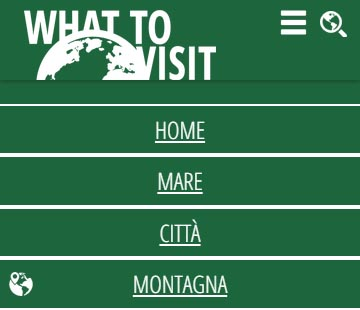
\includegraphics[height=4.65cm,width=5.4cm]{images/pres_nav_m.jpg}
                \caption{Navigation Menù su Dispositivi Mobili}
                \label{fig:Nav-mobile}
        \end{subfigure}
        \caption{Gli Header di WTV}\label{fig:Display-Header}
\end{figure}

